\chapter{Descripción del problema}
\label{chap:descripcion}

El presente trabajo intentará responder entonces a: ¿La entropía mejora las
posibilidades de marcar gol? Si cambia la entropía del equipo, ¿podemos
determinar la causa?¿Ha sido por un jugador específico, la alineación o más bien
la influencia del equipo contrario?. Igualmente, ¿es posible ver la entropía
reflejada en un tipo de visualización de las redes de pases?. Estudiaremos hasta
qué punto es determinante la entropía a nivel de jugador o equipo, empleando
técnicas estadísticas para obtener respuestas a lo planteado y siguiendo la
forma de trabajar que pasamos a describir.

\section{Metodología - Desarrollo ágil}
La metodología nos dicta dos cosas esenciales:
\begin{enumerate}
    \item ¿Qué tengo que hacer ahora?
    \item ¿Lo que he hecho está bien y era lo que tenía que hacer?
\end{enumerate}

Para el primer punto, hacemos uso de \textit{issues} y \textit{milestones} en Github, 
como veremos más adelante. Para lo segundo, hay que tener en cuenta que todos 
los \textit{issues} son problemas, e idealmente deben de decir explícitamente 
(o implícitamente si está claro) cómo se resuelve el problema.

El desarrollo ágil tiene su origen en el manifesto ágil\cite{manifiesto-agil},
el cual fue una revolución frente al modelo en cascada, en la forma de
desarrollar software, y planteaba que tienen más valor las personas que los
procesos o herramientas, un producto funcionando que mucha documentación,
colaboración con los clientes que contratos, y \textbf{flexibilidad} frente a
seguir un plan. Desde el año 2001 que se redactó ha cambiado mucho la
tecnología, y por ejemplo nosotros pondremos mucho peso en la documentación, mas
la idea sigue intacta: lo importante son los usuarios, adaptarse a sus
deseos. En general pues, con \textit{ágil} nos referimos a una forma de pensar
que se aplica a todo un ciclo de desarrollo del software centrado en el cliente
y que consiste en continuas mejoras de productos mínimamente
viables\cite{agile-science}.  En este apartado entenderemos mejor y dejaremos
claro lo que esto significa e implica.

Lo esencial de esta forma de proceder es que su objetivo es \textbf{resolver problemas} y satisfacer 
al cliente, no hacer aplicaciones: importa el por qué, antes que el qué o el cómo. Estos 
últimos resultarán de ese primer análisis, seguidos de una empatización, que consiste 
en contactar con clientes, leer prensa y demás para enfocar el problema; posteriormente 
ideación, de la que saldrán los objetivo e hitos o historias de usuario; y por último diseño, 
que será aterrizar todo lo anterior. 

Consecuentemente, el punto de partida es pensar la motivación o problema que queremos resolver. 
¿Por qué queremos hacer este TFG? ¿A quién ayuda? ¿Quién lo usaría? ¿Qué solución proponemos? 
Los problemas deben estar antes que nada; es complicado comprar ingredientes si no sabes qué 
receta vas a preparar. 

Luego, de la motivación saldrán los objetivos que nos planteamos. Estos habrán de indicar 
qué es lo que se quiere conseguir, incluyendo qué tipo de medios tenemos disponibles. Lo 
más importante es que han de estar en el dominio del problema, tienen que ser específicos, 
medibles y alcanzables\cite{objetivos}. De estos objetivos saldrán una serie de productos 
mínimamente viables. 

Seguidamente, las \href{https://jj.github.io/curso-tdd/temas/dise%C3%B1o.html}{historias de usuario} sirven 
para centrarnos en los problemas que queremos solucionar 
y los objetivos a alcanzar. Están relacionadas con la lógica de 
negocio del proyecto y siempre son un beneficio para los posibles usuarios del proyecto.

Una regla del pulgar para las historias de usuario: Siempre tienen que expresar un deseo y un 
beneficio para el usuario. Si ponemos ``ojalá qué" y te lo imaginas en la boca del usuario y suena 
creíble, es que es una historia de usuario. Si no, es un \textit{issue} o tarea que necesitamos
que el usuario haga para que cumpla sus deseos. El problema reside en poner lo que nosotros queremos que 
haga el usuario para conseguir algo, y no lo que el usuario quiere. Más adelante expondremos las historias 
de usuario planteadas.

Por otro lado, las \href{https://docs.github.com/articles/about-issues}{issues} plantean un problema. 
Siempre están enmarcadas en una \href{https://docs.github.com/en/issues/using-labels-and-milestones-to-track-work/about-milestones}{milestone}, 
y tienen que tener un criterio de aceptación para ser cerradas. Hacer tareas lo más atómicas posibles ayuda, porque 
se hace un \href{https://docs.github.com/en/pull-requests/collaborating-with-pull-requests/proposing-changes-to-your-work-with-pull-requests/about-pull-requests}{pull request}, 
se termina una tarea, y se avanza más fácil y suavemente.

Todo el código se incorpora mediante \textit{pull requests}, eventos que ocurren cuando un contribuidor está 
preparado para iniciar el proceso de mezclar el nuevo código, normalmente desarrollado en una \href{https://docs.github.com/github/collaborating-with-issues-and-pull-requests/about-branches}{rama}, 
con el repositorio del proyecto principal. Facilita así la revisión por parte de otra persona del equipo, y el 
asegurarnos de que en producción siempre hay algo que funciona y está testeado.

De manera adicional, un \textit{milestone} describe un producto mínimamente viable, y el estado en el que tiene 
que estar el repositorio al terminar, además de los criterios que se daben seguir 
para validarlo.

Dentro de la metodología descrita, nos enmarcaremos en el \href{https://www.iebschool.com/blog/design-thinking-agile-scrum/}{design thinking}, 
un proceso iterativo y no lineal que consta de una fase inicial consistente en empatizar con el 
cliente, para saber qué necesita, seguida de la definición del problema, pensar en una solución al 
mismo, el desarrollo de un prototipo, y finalmente se testea todo. 

\section{Herramientas usadas}
En esta sección profundizaremos en las herramientas empleadas para desarrollar el trabajo y seguir 
la metodología ya descrita, además de explicitar por qué las hemos escogido.

\subsection{Plataforma de desarrollo} 
Necesitábamos una plataforma que nos permitiera guardar el proyecto en algún sitio aparte de nuestro 
ordenador, para que en caso de problemas con el mismo pudiéramos continuar el desarrollo y no perderlo 
todo, a la vez que consultar versiones anteriores de lo escrito, dado que en algunas ocasiones se borran 
cosas que luego quieres incluir, o simplemente surge la necesidad de consultar el estado del trabajo en 
otro momento, para restablecerlo incluso. Es esencial tener un visión global de la construcción paso a paso 
de lo desarrollado, así como ver quién ha aportado qué, permitir que se sugieran cambios o añadan comentarios 
de una manera fácil, sin tener que andar pasando \textit{zips} para arriba y para abajo. Teniendo en consideración 
el potencial tamaño de un proyecto como el que nos ocupa, es importante también que a la plataforma ``no le importe'', 
siga funcionando rápido y no limite de ninguna manera lo que se tiene pensado hacer, sino más bien lo haga sencillo, 
intuitivo, \textit{disfrutable}. Sin tener que instalar \textit{gigas} de paquetes ni nada, tan solo sea una parte 
más y se funda con el proyecto. Por supuesto, que sea gratuita es un buen añadido, al igual que el que tenga 
una gran comunidad detrás. Todo esto nos llevó a escoger \href{https://github.com/}{Github} (y seguro que nos 
dejamos algo; GitHub ofrece increíbles posibilidades).

Github es una aplicación con web (también API o marco de aplicaciones, entre otras) muy completa 
para que desarrolladores y programadores puedan trabajar colaborativamente 
en repositorios. Su punto fuerte es el sistema de control de versiones, que permite llevar 
cuenta detallada de los cambios realizados por cada persona, discutirlos, revisarlos y proponer 
modificaciones, así como 
separar el producto final de las funcionalidades que se vayan añadiendo y sobre las que cada equipo o persona 
esté trabajando, mediante \href{https://docs.github.com/pull-requests/collaborating-with-pull-requests/proposing-changes-to-your-work-with-pull-requests/about-branches}{ramas}. 
Adicionalmente, proporciona herramientas como las \href{https://github.com/features/actions}{Github Actions}, 
las cuales permiten la automatización de los flujos de trabajo, incluyendo integración y despliegue contínuos.
Nosotros por ejemplo lo empleamos para chequear la ortografía cada vez que subimos algo al repositorio, o construir el \textit{pdf}
de la memoria cuando se cambie algún archivo \textit{.tex}, pero por supuesto hay muchísimas más funcionalidades posibles.

Se puede consultar nuestro repositorio en \href{https://github.com/ElenaMerelo/TFG}{el siguiente enlace}, y navegar 
por las \href{https://github.com/ElenaMerelo/TFG/issues}{issues creadas}, \href{https://github.com/ElenaMerelo/TFG/pulls}{pull requests mergeados} 
o \href{https://github.com/ElenaMerelo/TFG/actions}{actions usadas}. Para el desarrollo de nuestro trabajo es esencial 
Github, y lo hemos escogido por ser de los más usados y establecidos, con más de 45 millones de usuarios, 
y porque frente a \href{https://about.gitlab.com/}{gitlab}, contiene justo lo que necesitamos. Gitlab es para proyectos 
más grandes y profesionales.

Para tener conciencia situacional del estado del repositorio de Github, instalamos \href{https://ohmyz.sh/}{oh my zsh}, 
un \textit{framework} libre para administrar la configuración del \textit{shell} \textit{Zsh}. Permite el 
acceso y fácil instalación de plantillas para la terminal, que hacen más fácil saber en qué rama se está 
trabajando, qué cambios se han realizado, si están ya añadidos o no, y en general casa genial con 
\textit{Github} y sus funcionalidades. Tiene detrás una comunidad muy grande de 
contribuidores, incluye numerosos \textit{plugins} que hacen el desarrollo de \textit{software} más fácil y bonito, 
y la posibilidad de personalizar la terminal, con temas ya creados o propios.

Añadir que {Zsh} es un \textit{shell} que se presenta como alternativa a \textit{bash}, el cual viene por defecto en 
\textit{Ubuntu}. Las ventajas de las que más nos hemos aprovechado y por las que lo escogimos parten de 
su mayor configurabilidad, el que te corrija errores de escritura y complete palabras, y esa necesidad que ya 
hemos mencionado de tener un buen conocimiento de la situación y el desarrollo.

\begin{figure}[h!]
    \centering
     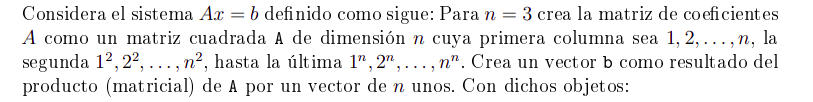
\includegraphics[width=\textwidth]{./img/ohmyzsh.png}
     \caption{Cómo se ve nuestra terminal}
     \label{img:dag1}
\end{figure}


\subsection{IDE}
Como editor de código precisábamos de uno que diera soporte a varios lenguajes de programación, fuera bien en 
Ubuntu, se pudiera coordinar con Github sin problemas, hiciera la escritura de código algo más fácil con 
funcionalidades como autocompletación de palabras, resaltado de código y corchetes, autoindentación, herramientas de 
compilación o \textit{debugging}, seguimiento de definiciones, atajos de teclado o un mercado de plugins y temas 
para facilitar lo anterior, y más en general hacer sencillo el desarrollo. Por ello su enorme potencial y comunidad 
detrás, escogimos \href{https://code.visualstudio.com/}{Visual Studio Code}. Combina pues la simplicidad 
de un editor de código fuente con herramientas de desarrollo potentes, como completación de código o 
\textit{debugging}. Y lo mejor, es software libre, y se integra perfectamente con git y Github, además de 
permitirte construir el proyecto y compilarlo, todo sin cambiar de pantalla ni rompederos de cabeza; es intuitivo 
y hasta diríamos inteligente.

Como opciones, destacamos \href{https://netbeans.apache.org/}{Apache Netbeans}, 
\href{https://www.eclipse.org/downloads/}{Eclipse}, \href{https://www.rstudio.com/}{RStudio}, \href{https://www.vim.org/}{Vim} o 
\href{https://www.gnu.org/s/emacs/}{Emacs}. De todos ellos, es el que mejor puntuación y \textit{reviews} tiene 
en la web. Lo elegimos antes que Netbeans dado que este no se puede integrar con Github, el desarrollo es más 
personalizado y permite revisión de código o seguimiento de errores; se ajusta más que Netbeans para lo que 
queremos hacer y es más fácil de usar, con mayor número de funcionalidades. VS Code es más eficiente que Vim, y 
gana con diferencia, al ser un IDE completo y no solo un editor de textos, en el que habría que hacerlo casi 
todo a mano. Por supuesto, hay muchos puristas de Vim o Emacs, que ya han pasado el periodo de adaptación y saben 
usarlo genial, lo tienen chetadísimo, pero las ventajas y características de VS Code hacen que nos quedemos 
con él, aparte de la ya reiterada estupenda integración con Github de la que estos últimos carecen. Por último, 
hemos incluido RStudio debido a que la parte informática será en ese lenguaje, y para ello es maravilloso, pero 
desde VS Code también se puede hacer, así que mejor tenerlo todo centralizado.

\subsection{Lenguaje de programación}
% Igual, enumera las posibilidades, los requisitos, y escoge uno.
Escogimos \href{https://www.r-project.org/}{R} puesto que necesitábamos un lenguaje que no nos pusiera límites 
en cuanto a la aplicación de la teoría matemática, esto es, fuera bueno para estadística computacional y 
análisis, permitiera realizar gráficos, y constara de numerosos paquetes, una gran comunidad detrás, 
fuera gratis y software libre, además de que llevara muchos años asentado como herramienta de desarrollo, y en 
continua expansión y crecimiento.

\subsection{Sistema de composición de documentos}
%mencionar quarto
\href{https://www.latex-project.org/}{LaTeX} es un sistema estándar para la composición de documentos 
científicos y técnicos, software libre y gratuito. Lo escogimos ante la necesidad de un programa que nos 
permitiera escribir la memoria, con soporte para lenguaje matemático o código informático, sin tener que 
andar ajustando tamaños de letras, imágenes o índices. Queríamos centrarnos en el contenido, y no tanto 
en el formato. En un principio, puede parecer más fácil usar Word o LibreOffice, pero para escribir proyectos 
más grandes que no comprendan únicamente texto, tras una pequeña fase de aprendizaje, LaTeX gana con ventaja, 
al disponer también de plantillas, una documentación excelente, y años y años de consolidación en la comunidad 
científica. 

LaTeX da pues al usuario un control extremadamente bueno sobre el formato de los documentos. Una vez que se 
domina, puede ser mucho más fácil trabajar con él que con un procesador de texto convencional. Tuve 
problemas (que fui reflejando en \href{https://github.com/ElenaMerelo/TFG/issues}{mi Github}) a la hora 
de usarlo ya que no lo había empleado hasta este momento, por lo que tenía que entender 
el funcionamiento de la plantilla que uso, \href{https://github.com/ElenaMerelo/TFG/issues/58}{cómo escribir las fórmulas 
y símbolos matemáticos}, \href{https://github.com/ElenaMerelo/TFG/issues/54}{la definición de entornos}, 
\href{https://github.com/ElenaMerelo/TFG/issues/56}{cómo hacer citas y referencias}, 
\href{https://github.com/ElenaMerelo/TFG/issues/57}{cómo se incluyen imágenes}, cómo incluir y usar paquetes, 
o incluso cómo poner títulos, letra 
en itálica, enlaces. Hay numerosos tutoriales en internet, pero lo que más consulté ha sido
 \href{https://es.overleaf.com/learn}{la documentación de Overleaf}, aunque tenga otro editor de LaTeX. Ciertamente, 
 la curva de aprendizaje no es muy grande, y una vez entiendes la lógica detrás, se escribe relativamente rápido. En 
 cualquier caso, es mejor que ir buscando la fórmula en el cuadro de mandos de los editores de texto tradicionales, 
 y al ser ficheros de texto los edito en VisualCode Studio y puedo subirlos al repositorio de GitHub junto con el resto 
 del proyecto. 

\section{Clientes}
Basándonos en la \href{https://www.designthinking.services/herramientas-design-thinking/metodo-persona/}{metodología basada en personas}, 
hemos llegado a los siguientes usuarios \footnote{Para más información sobre las
  figuras que aparecen en el análisis de datos deportivos, consultar
  \href{https://objetivoanalista.com}{Objetivo Analista}}:
\begin{itemize}
    \item Analista táctico: estudia los equipos y cómo se desenvuelven en los partidos. 
    \item {\em Scouter}: en algunos equipos grandes existe esta figura que asiste a
      encuentros de otras ligas, otras divisiones, o incluso el filial, para
      identificar qué jugadores pueden entrar en los planes de adquisición o de
      ascenso a equipos de categorías superiores del club.
    \item Analistas de datos: tienen que generar la estrategia de recogida de
      datos del club y preparar aplicaciones e informes para ayudar en la toma de
      decisiones del mismo.
    \item Persona que apuesta: recopila información sobre los equipos y jugadores, para poder apostar 
    en base a una alineación, o una vez se sabe quién va a jugar en un partido. 
    \item Entrenador: es el encargado de decidir a quién sacar durante un partido, los 
    cambios, dónde poner a quién. 
    \item Presidente del equipo de fútbol: tiene que decidir antes del comienzo 
    de cada temporada cuánto dinero ha de invertir en nuevos jugadores. 
    \item Periodista deportivo: debe escribir un artículo sobre un partido con gráficos y datos estadísticos, 
    para lo que debe conocer medianamente a los jugadores y equipos, junto con su desempeño a lo largo de 
    una liga o temporada. 
\end{itemize}

\section{Historias de usuario}  

A partir de los clientes, y como parte de la metodología, definimos en \href{https://github.com/ElenaMerelo/TFG/issues?q=is%3Aopen+is%3Aissue+label%3Auser-story}{las siguientes historias de usuario}: 

\begin{itemize}
    \item Como analista táctico, quiero obtener un análisis del propio equipo y de los rivales.
    \item Como scouter, quiero tener elementos cuantitativos de juicio, a partir
      de las observaciones, para tomar decisiones que beneficien el desempeño
      deportivo del club.
    \item Como analista de datos, deseo conocer qué metodología de obtención,
      tratamiento y presentación de datos es la que me permite elaborarlos con
      más claridad para presentarlos a los que toman las decisiones en el club.
    \item Como persona que apuesta, querré inferir el resultado de un partido y 
    quién marcará, una vez se publiquen los jugadores. 
    \item Como entrenador, me gustaría poder usar la herramienta desarrollada, y que sea intuitiva.
    \item \label{hu:presidente} Como presidente del equipo de fútbol, quiero poder calcular los ingresos 
    probables por las ventas de jugadores no deseados, el gasto neto relativo de otros
    equipos y el posible impacto negativo en el desempeño del equipo de hacer demasiados cambios de personal de una 
    vez.  
    \item Como periodista deportivo, desearía tener una herramienta más en mi arsenal, y 
    usarla para obtener gráficos, estadísticas, y conclusiones acerca de un partido, 
    temporada, equipo o jugador.
    \item Como tutores, nos gustaría que el proyecto siga un desarrollo ágil.
    \item Como matemática, quiero que la teoría sobre redes causales se aplique bien al caso concreto, y 
    se conecte sin problema con la parte informática.
\end{itemize}

\section{Hitos o Productos Mínimamente Viables}
Pasamos a describir los prototipos del producto que queremos desarrollar.

\subsection{\textit{Milestone} 1 - Infraestructura}
El objetivo de esta \textit{milestone} es configurar la infraestructura del proyecto. Para ello, tendremos que:
\begin{itemize}
    \item Borrar los archivos de la plantilla que no sean necesarios.
    \item Definir los primeros \textit{milestone} e issues.
    \item Configurar un corrector ortográfico.
    \item Documentar la configuración inicial.
    \item Formular los objetivos principales del trabajo.
\end{itemize} 
De esta manera, tendremos hecho el esqueleto sobre el que seguir construyendo. El objetivo principal y 
producto esperado de este \textit{milestone} es pues tener claro el problema a resolver y los objetivos 
de este trabajo.
   
Al final de esta milestone, se pretende tener el repositorio configurado de forma que tengamos las 
bases para crear un producto de calidad (sin faltas ortográficas, por ejemplo).

\subsection{\textit{Milestone} 2 - Planteamiento}
El objetivo de esta \textit{milestone} es dejar escritas:

\begin{itemize}
    \item Introducción
    \item Descripción del problema
    \item Estado del arte
    \item Planificación
    \item Metodología
    \item Clientes, usuarios e historias de usuario
\end{itemize}

Habiendo terminado así la parte de ideación, planteamiento del problema, y pasar a estar preparado para solucionarlo.

\subsection{\textit{Milestone} 3 - Parte matemática} 
El objetivo de esta \textit{Milestone} es la recopilación de datos, procesarlos, eliminar los que 
no sirvan, obtener conclusiones. Aparte, habría que reproducir teoremas, dejar bien clara la base matemática.

Como producto esperado se tendrá la base teórica terminada y bien explicada, para ello habrá que: 

\begin{itemize}
    \item Añadir fundamentos de redes
    \item Incluir fundamentos de probabilidad 
    \item Añadir fundamentos de redes probabilísticas 
    \item Entender cómo se pueden resolver redes probabilísticas 
    \item Añadir introducción a las redes causales 
\end{itemize}

\section{Definiciones y terminología}
El objetivo de esta sección es introducir los términos que serán usados en el estado del arte, donde veremos 
todavía mejor cómo se conectan con nuestro problema.

Enunciamos en primer lugar lo que son los modelos gráficos probabilísticos, ya que permiten realizar 
inferencia en dominios complejos dotados de incertidumbre.

\begin{definicion}{Modelos gráficos probabilísticos} \label{subsect:modelos}
Un modelo gráfico probabilístico es una representación de la distribución de probabilidad conjunta 
sobre un dominio, que consta de dos partes: una componente cualitativa
en forma de grafo que codifica afirmaciones de independencia condicional sobre el 
dominio que se está estudiando, y una componente cuantitativa que consiste en una colección de 
distribuciones de probabilidad locales que cumplen la propiedades de independencia especificadas 
en el modelo \cite{inference-rev-hbn}. 
\end{definicion}

Un tipo de modelo gráfico probabilístico que usaremos y estudiaremos en profundidad en los próximos 
capítulos son las redes bayesianas.

\subsection{Redes bayesianas} \label{subsect: BN}
\begin{definicion}[Redes bayesianas] \label{def:BN}
Una red bayesiana \cite{def-bncn} $\mathfrak{B} = \lbrace \mathcal{G}, \mathbb{P} \rbrace$ está definida por:
\begin{itemize}
    \item Un grafo dirigido acíclico $\mathcal{G}=(V,E)$ donde $V$ es un conjunto de nodos y $E$ 
    es un conjunto de aristas.
    \item Un espacio de probabilidad $(\Omega, \mathbb{P})$.
    \item Un conjunto de variables aleatorias $\textbf{V}=V[i], i=1,...,N$ con N lista de variables aleatorias, 
    asociadas con los nodos del grafo $(\Omega, \mathbb{P})$ 
    de tal manera que $\mathbb{P}(V[1],...,V[N])= \prod_{i=1}^{n}\mathbb{P}(V[i]|pa(V[i]))$, donde $pa(V[i])$ es el 
    conjunto de los nodos padre de $V[i]$ en $\mathcal{G}$.  
\end{itemize}
\end{definicion} 

En otras palabras, una red bayesiana es un grafo donde los nodos representan variables aleatorias discretas 
o contínuas y los bordes o aristas representan las influencias entre ellas. Las aristas 
representan pues las causalidades, que pueden ser determinísticas o probabilísticas. Para un borde 
uniendo el hecho $A$ con el $B$, con $P(B|A)$ representamos la relación de probabilidad de un 
nodo, conocidos sus padres. Para los nodos sin padres o nodos raíz, se asignará una probabilidad previa.

Vamos a ver un poco más específicamente qué queremos decir cuando hablamos de grafos.
\subsubsection{Grafos}
\begin{definicion} \label{def:grafo}
Un grafo es un par $\mathcal{G} = (V, E)$, donde $V$ es un conjunto finito de vértices distinguibles y 
$E \subseteq V \times V$ es un conjunto de aristas. Un par ordenado $(u, v) \in E$ denota un borde dirigido
del vértice $u$ al vértice $v$, y se dice que $u$ es padre de $v$ y $v$ hijo de $u$. Al conjunto de padres 
e hijos de un vértice $v$ los denotaremos por $pa(v)$ y $ch(v)$, respectivamente. Los bordes dirigidos 
se representarán con flechas, y los bordes no dirigidos con líneas. 
\end{definicion}

\begin{figure}[h!]
    \centering
     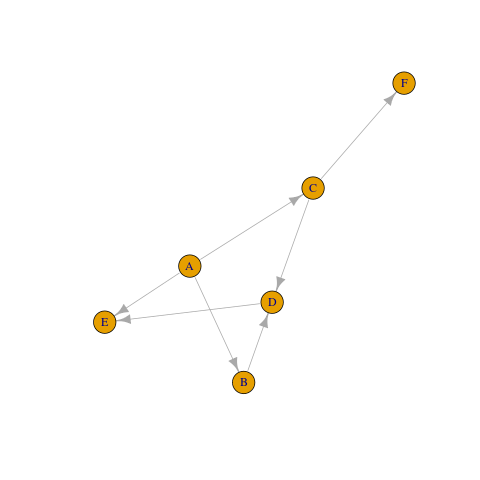
\includegraphics[width=\textwidth]{./img/dag.png}
     \caption{Ejemplo de grafo dirigido acíclico (DAG). Generado mediante \href{https://github.com/ElenaMerelo/TFG/blob/master/scripts/dag.R}{un script en R}.}
     \label{img:dag1}
\end{figure}

Un camino $ \langle v_{1},...,v_{n} \rangle $ 
es una secuencia de vértices distinguibles tales que $u \rightarrow v$, $v \rightarrow u$ o $u - v$ para 
cada $i= 1,..., N-1$. El camino es dirigido si $v_{i} \rightarrow v_{i+1}$ 
para cada $i= 1,..., N-1$; $v_{i}$ es por tanto un ancestro de $v_{j}$ y $v_{j}$ es un descendiente de 
$v_{i}$ para cada $j > i$. 

Un ciclo es un camino, $\langle u,...,v \rangle$ de longitud mayor que dos 
(excepto el caso $v_{1} = v_{N}$); un grafo 
dirigido sin ciclos dirigidos es el ya mencionado DAG. 

Generalmente, las redes bayesianas se utilizan como un marco eficiente para la
toma de decisiones con conocimiento incierto, y mide la estructura de dependencia condicional
de un conjunto de variables aleatorias basándose en el teorema de Bayes:\\
\begin{equation} \label{eq:bayes}
P(A|B) = \frac{P(B|A) \cdot P(A)}{P(B)}
\end{equation}
donde $P(A)$ es la probabilidad previa, $P(B)$ son las observaciones y la probabilidad posterior viene dada 
por $P(A|B)$ \cite{YANG201919}.

En \ref{ch5} profundizaremos más sobre este tipo de redes.

En aplicaciones prácticas, es común encontrar escenarios que
involucran variables discretas y continuas simultáneamente. Este tipo de problemas se pueden modelar 
utilizando las llamadas redes bayesianas híbridas.

\subsection{Redes bayesianas híbridas}
\begin{definicion}[Redes bayesianas híbridas] \label{def:hybrid_BN}
    Una red bayesiana híbrida \cite{hybrid-BN} es un tipo de red bayesiana que permite modelar incertidumbre
    sobre variables discretas y contínuas.
\end{definicion}

Han recibido una atención creciente durante 
los últimos años, debido a que amplían la aplicabilidad de las redes bayesianas en general. Sin embargo, 
esta característica adicional también tiene un costo: la inferencia
en este tipo de modelos es computacionalmente más desafiante \cite{inference-rev-hbn}.

Tradicionalmente se han aplicado más las redes complejas que las bayesianas al análisis del fútbol \cite{ARRIAZAARDILES2018236}.
Este tipo de redes nos interesan ya que su estudio está inspirado por los análisis empíricos de redes reales, y 
permiten entender el funcionamiento de los equipos de fútbol, ya sea a nivel individual o colectivo. Usaremos 
variables definidas sobre la red compleja para ``alimentar" la red bayesiana \cite{Bai_Xing_Wu_2022}.

\subsection{Redes complejas}
\begin{definicion}[Redes complejas] \label{def:CN}
    Una \href{https://en.wikipedia.org/wiki/Complex_network}{red compleja} 
    es un grafo con características topológicas que no se dan 
    en redes simples como \href{https://en.wikipedia.org/wiki/Lattice_(order)}{celosías} o 
    \href{https://mathworld.wolfram.com/RandomGraph.html}{grafos aleatorios}, pero a menudo ocurren en redes que 
    representan sistemas reales. 
\end{definicion}

Estos sistemas son llamados complejos debido a que no es posible predecir directamente su 
comportamiento colectivo a partir de sus componentes individuales. Una de las principales razones por las que 
las redes complejas son populares es su flexibilidad
y generalidad para representar prácticamente cualquier estructura natural, incluidas las que experimentan 
cambios dinámicos de topología \cite{CN-review}.

La teoría de redes complejas se desarrolla en base a la teoría de grafos y la física estadística; en esta, 
todo sistema complejo puede abstraerse como una red. Los nodos de la red se pueden 
considerar como los elementos en el sistema, y las relaciones
entre cada elemento como conexiones. Hay muchos indicadores estructurales
en la teoría de redes complejas que pueden cuantificar la importancia de los nodos desde el nodo mismo o el
nivel de relación de red, usando \href{https://link.springer.com/10.1007%2F978-1-4419-9863-7_935}{centralidad de grado}, 
\href{https://neo4j.com/docs/graph-data-science/current/algorithms/eigenvector-centrality/}{centralidad de vectores propios} 
y \href{https://en.wikipedia.org/wiki/Clustering_coefficient}{coeficiente de agrupamiento} \cite{albert2002statistical}.
 


Otra manera de medir la importancia de cada nodo es mediante sistemas de calificación.

\subsection{Sistemas de calificación} \label{subsect:ratings}
Determinar la habilidad relativa entre adversarios es uno de los elementos
más importantes en el análisis de fútbol junto con la predicción de resultados de partidos de fútbol; las posiciones en 
una liga constan de numerosos inconvenientes que hacen que no sean fiables para la predicción. 
Por ejemplo, una liga de fútbol sufre de alta variación al inicio de la temporada, y de baja 
variación al final. Además, es posible que los equipos que compiten durante una temporada no
compartan un número equivalente de partidos jugados debido a aplazamientos y
por lo tanto, la clasificación de la liga será errónea durante unas cuantas semanas. De hecho, 
la clasificación de una liga está sesgada hasta que se juega el último partido de la temporada, porque
para que la clasificación sea justa, cada equipo tiene que jugar contra el resto de equipos, en
casa y fuera. Incluso al final de una temporada, el \textit{ranking} representa
el rendimiento general durante ese período, pero no logra
demostrar cómo varió la habilidad de un equipo. Adicionalmente,
ignora los partidos de Copa y los partidos de otras competiciones (por ejemplo, Champions
League), o no compara equipos en diferentes divisiones/ligas. \textbf{En
resumen, una tabla de clasificación no es un buen indicador de la situación actual de un equipo. Un 
sistema de calificación proporciona medidas relativas de superioridad entre adversarios y supera 
todos los problemas anteriores \cite{pi-ratings}.}

Cuando se trata de fútbol, para generar calificaciones que capturen con precisión la
capacidad actual de un equipo, tenemos que considerar al menos:
\begin{itemize}
    \item La ventaja que supone jugar en casa.
    \item El hecho de que los resultados más recientes son más importantes que los menos recientes
    al estimar las habilidades actuales.
    \item El hecho de que una victoria es más importante para un equipo que aumentar la diferencia de goles.
\end{itemize}

\begin{definicion} \label{def:ratings}
La calificación general de un equipo es la calificación promedio entre las actuaciones 
en casa y fuera, y esto se define como

$$ R_{\tau}= \frac{R_{\tau H} + R_{\tau A}}{2} $$

donde $R_{\tau}$ es la calificación para un equipo $\tau$, $R_{\tau H}$ es la calificación para el 
equipo $\tau$ cuando juega en casa, y $R_{\tau A}$ es la calificación de un equipo $\tau$ cuando 
juegan fuera. 
\end{definicion}

Nosotros calificaremos a los equipos según su entropía.

\subsection{Entropía}
La entropía es el concepto clave para extraer características universales de un sistema a partir de sus 
detalles. Aparece en muchos contextos como termodinámica, mecánica estadística o teoría de la información, como 
una medida de diferentes propiedades: energía que no puede producir trabajo, nivel promedio de información, sorpresa, 
desorden, incertidumbre, aleatoriedad o complejidad \cite{gen-entr-review}, \cite{t-entropy}.

\begin{definicion}[Entropía] \label{def:entropy}
Para una variable aleatoria discreta $X$ definimos su entropía como:  

$$H(X):= - \sum_{x} P(x)\log[P(x)]$$

bits, donde $X$ toma valores en $\mathcal{X}$, $P:\mathcal{X} \rightarrow [0,1]$, $P(x)$ es la 
probabilidad de que $X$ esté en el estado $x$. La 
entropía conjunta de las variables $X_1...X_N$ se define por 
$$H(X_1,...,X_N)=-\sum_{x_1}...\sum_{x_N}P(x_1,...,x_N)\log[P(x_1,...,x_N)]$$
\end{definicion}

El concepto de entropía (o entropía de Shannon) se lo debemos al matemático e ingeniero eléctrico americano 
\href{https://en.wikipedia.org/wiki/Claude_Shannon}{Claude Shannon}, que lo introdubjo en 1948 en el 
artículo ``Una teoría matemática de la comunicación" \cite{shannon-1948}.

La entropía que más nos interesa es la de Tsallis, al ser la que se puede aplicar mejor a las redes de pases 
que ocurren a lo largo de un partido de fútbol
\subsection{Entropía de Tsallis}
En 1988 el físico \href{https://en.wikipedia.org/wiki/Constantino_Tsallis}{Constantino Tsallis} 
introdujo una nueva definición para entropía que describe las características estadísticas de sistemas 
complejos. Fue diseñada para analizar sistemas donde existen correlaciones entre sus microestados \cite{tsallis}.
\begin{definicion}[Entropía de Tsallis] \label{def:tsallis_entropy}
Dado un conjunto discreto de probabilidades ${p_i}$ con la condición $\sum_{i} p_i = 1$, y con $q$ 
cualquier número real, se define la entropía de Tsallis como
$$ S_q(p_i)=\frac{k}{q-1}\left(1- \sum_{i=1}^{N}p_{i}^{q}\right)$$
donde $q$ se denomina índice entrópico, $N$ son los microestados y $k$ es una constante positiva.
\end{definicion}

La fórmula se reduce a la de la entropía de Shannon cuando $q=1$. En último lugar, notar que si se 
combinan dos sistemas idénticos, 
la entropía de Tsallis del sistema combinado no es igual a la suma de la entropía de sus 
subsistemas \cite{comparison-entropies}. Esto quiere decirnos que podemos trabajar con la entropía de 
alguna variable calculada a partir de los jugadores.
